
\documentclass[11pt,journal]{RapportFR}

\usepackage{textcomp}

\usepackage{CJK}
\usepackage[overlap,CJK]{ruby}    % Furigana support
\renewcommand{\rubysize}{0.5}     % Furigana size
\renewcommand{\rubysep}{-0.3ex}   % Spacing between Furigana and Kanji



\usepackage[dvips]{graphicx}
\graphicspath{{./Photos/}}
\DeclareGraphicsExtensions{.eps}



% correct bad hyphenation here
\hyphenation{op-tical net-works semi-conduc-tor}


\begin{document}
\begin{CJK*}{UTF8}{min}

\title{Rapport Culturel - Japon 2011}


\author{L\'{e}o Baudouin.
%\thanks{Un grand merci \`a Nicolas Perrin, Olivier Stasse, Eichii Yoshida, Thomas Moulard et toutes les personnes que j'ai pu rencontrer pendant ce voyage.}
}

% The paper headers
\markboth{IFMA}{Shell \MakeLowercase{\textit{et al.}}: Rapport culturel sur mon stage au Japon.}

\maketitle


\begin{abstract}
\boldmath
Ce rapport est un compte-rendu des observations sur le Japon et les Japonais concernant leur mode de vie et leurs comportements, ainsi qu'une br\`eve analyse critique des diff\'erences entre les Fran\c cais et les Japonais. Il mentionne \'egalement l'incident survenu au large des c\^otes japonaises en mars 2011.

\end{abstract}

\begin{IEEEkeywords}
Stage \`a l'\'etranger, Japon, AIST, rapport culturel.
\end{IEEEkeywords}



\section{Introduction}


\IEEEPARstart{U}{n} des buts des stages \`a l'\'etranger propos\'es par l'IFMA dans le cadre d'une ann\'ee de c\'esure est de d\'ecouvrir, de visiter un pays, de comprendre ses habitants et d'apprendre sa langue.
L'objectif culturel de ce stage \'etait de s'impr\'egner de la culture japonaise, et donc de confirmer ou non les id\'ees re\c cues que j'avais sur les habitants du pays du soleil levant.

J'ai effectu\'e mon stage \`a Tsukuba (つくば市), dans la pr\'efecture d'Ibaraki, au nord-est de Tokyo, dans le laboratoire japonais AIST -- Advanced Industrial Science and Technology. La section dans laquelle j'ai travaill\'e, le JRL -- Joint Robotic Laboratory, \'etait compos\'ee de quelques Japonais et d'une dizaine de Fran\c cais. L'anglais \'etait donc la langue officielle lors des r\'eunions ou pour les rapports. 


Avant de partir, j'avais, comme tout le monde, une id\'ee pr\'econ\c cue du Japon : un pays riche en avance sur son temps, un paradis de la technologie. J'avais \'egalement entendu que les Japonais faisaient souvent passer leur vie professionnelle avant la vie de famille. 
En allant au Japon je souhaitais d\'ecouvrir un monde nouveau, aussi bien au niveau de l'architecture, des paysages, du mode de vie et de la langue. Je voulais me plonger dans ce pays de la robotique et des technologies. 
%Au final seul la langue m'a vraiment d\'epays\'e, le reste \'etant assez semblable \`a la France.

Ce rapport commencera sur une partie consacr\'ee au Japon, en expliquant pourquoi j'ai choisi le Japon, et qu'elles ont \'et\'e les visites pr\'evues et r\'ealis\'ees pendant mon voyage. La section \ref{sec_mode_de_vie} d\'etaillera ce que j'ai pu voir au quotidien en vivant au Japon. Les principales contradictions constat\'ees seront expos\'ees dans la partie \ref{sec_contradictions}. Enfin, dans la partie \ref{sec_incident}, j'expliquerai ce qu'il est arriv\'e le 11 mars 2011 et pourquoi mon s\'ejour n'a dur\'e que 30 jours.



\section{Le Japon}

\begin{figure}[!t]
\centering
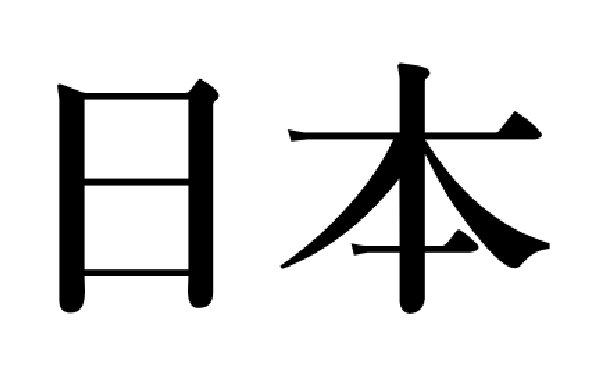
\includegraphics[width=3in]{nihon}
\caption{\textit{Nihon}, le Japon, \textit{lieu d'origine du soleil}.}
\label{fig_nihon}
\end{figure}

\subsection{Pourquoi le Japon}

Je n'\'etais jamais sorti de France avant de m'envoler pour ce pays \`a l'autre bout de la terre. Je voulais absolument partir loin afin de conna\^\i tre un d\'epaysement total, m\^eme si cela avait un petit c\^ot\'e effrayant pour moi.
Tout ce que je savais sur le Japon c'est qu'il a toujours \'et\'e consid\'er\'e comme un pays avec une culture unique au monde, un comportement et une vision des choses qui vont avec. Par ce voyage j'ai voulu en apprendre plus sur ce pays qui m'attirait depuis fort longtemps. Je voulais voir par moi m\^eme si ce pays \'etait aussi bien que le pr\'etendaient tous les reportages et DVD de voyages que j'ai pu voir. Je d\'esirais \'egalement d\'ecouvrir un autre mode de vie que le seul mode de vie occidental que je connaissais, afin de pouvoir tirer profit de chacun d'eux, je savais par avance que les 6 mois allaient \^etre beaucoup trop courts pour faire tout cela. 

J'ai \'egalement choisi le Japon car le sujet du stage qui m'\'etait propos\'e correspondait exactement \`a mon projet de carri\`ere, c'est \`a dire de la recherche dans le domaine de la robotique humano\"\i de. C'\'etait l'occasion pour moi de valider mon master recherche tout en travaillant avec le CNRS, en partenariat avec un laboratoire fran\c{c}ais, le LAAS, dans lequel j'envisage de faire une th\`ese. Commencer \`a travailler directement dans le pays qui est le mieux plac\'e dans ce domaine particulier ne pouvait \^etre qu'un avantage pour moi.

\subsection{Une langue complexe}

Pour pr\'eparer ce stage, j'avais pris des cours de japonais pendant plus d'un an. Ceux ci se sont av\'er\'es quasiment inutiles une fois en face d'un vrai Japonais, \'etant incapable de comprendre la r\'eponse \`a la question que je venais de bafouiller. Bien que le Japonais soit une langue assez simple \`a parler (construction logique des phrases, simplicit\'e de la grammaire et de la conjugaison), les Japonais ont tendance \`a parler vite, au m\^eme titre que les Espagnols et assez peu d'entre eux ne se soucient d'\^etre compris par les \'etrangers.

Ce qui a \'et\'e vraiment dur c'est l'\'ecriture car comme tout le monde le sait, le Japonais est plut\^ot indigeste. Il existe quatre fa\c{c}ons d'\'ecrire le japonais, deux syllabaires de base, les \textit{Hiragana} et les \textit{Katakana} (pour les mots d'origines \'etrang\`ere) comportant 46 syllabes chacun. Apr\`es un an d'apprentissage du japonais, je les comprenais sans difficult\'e. Cependant un troisi\`eme moyen d'\'ecrire le japonais existe, les \textit{Kanjis}, se sont des id\'eogrammes, qui repr\'esentent un mot ou une id\'ee. Il en existe 1975 officiels et plus de 3000 dans le langage courant, autant dire que les 20 ou 30 \`a ma connaissance n'ont \'et\'e d'aucune utilit\'e sur place. Une phrase typique japonaise m\'elange les \textit{Hiragana}, \textit{Katakana} et les \textit{Kanji}, donc il \'etait toujours impossible de lire une phrase enti\`erement. Le dernier moyen d'\'ecrire le japonais est le \textit{Romaji}, l'\'ecriture romaine des mots japonais, cependant celle-ci n'est utilis\'ee que pour les marques et les cours de japonais.
Il a donc \'et\'e tr\`es dur de s'y retrouver, aussi bien dans les restaurants que dans les magasins, car tr\`es peu d'articles sont doubl\'es en anglais ou en Romaji.

J'ai donc rapidement \'et\'e contraint de communiquer en anglais, et c'est \`a ce moment que j'ai pu me rendre compte que la plupart des Japonais ne le parlent pas ou tr\`es peu. J'ai essay\'e de poser mes questions aux \'etudiants pensant qu'ils auraient le m\^eme niveau que moi, mais sur un groupe de 5, seul un des Japonais parlait un anglais aussi h\'esitant que le mien. Les caissiers et caissi\`eres dans les magasins ne parlaient qu'en Japonais, il \'etait donc souvent tr\`es difficile de se comprendre et les gestes ne suffisaient pas tout le temps pour r\'esoudre les probl\'emes de compr\'ehension.

C'est seulement au laboratoire que j'ai pu rencontrer des Japonais parlant un anglais parfait, contrastant avec ceux que j'avais crois\'e en ville.
Je pensais que la France \'etait en retard sur l'apprentissage de l'anglais mais avec \'etonnement je me suis rendu compte que le Japon semble l'enseigner encore moins. 


\subsection{Visite du Japon}

Le Tsukuba Express dessert la gare d'Akihabara, dans le quartier "\'electrique" de Tokyo (東京). On y retrouve des centaines d'immenses magasins allant jusqu'\`a 8 ou 9 \'etages, ainsi que de minuscules boutiques sp\'ecialis\'ees dans l'\'lectronique(cf Photo \ref{fig_akihabara}).
Arriv\'e dans les rues d'Akihabara, ce qui m'a frapp\'e c'est le calme, \`a 9h les magasins sont ferm\'es et peu de gens circulent. Cependant \`a l'heure d'ouverture (10h), la ville s'est transform\'ee en fourmili\`ere, noire de monde. C'est \`a ce moment-l\`a que j'ai eu l'impression de revivre les documentaires sur le Japon.

Toutes les visites ont \'et\'e effectu\'ees avec ma compagne qui m'a accompagn\'e dans mon p\'eriple, je parlerai maintenant au pluriel quand il s'agira de remarques communes. C'est plus tard que nous avons retrouv\'e la m\^eme foule, en soir\'ee, dans le quartier de Shibuya (渋谷区), le quartier des jeunes. On y retrouve un grand nombre de magasins (v\^etement, musique, restaurant) \`a la mode et des \textit{Love Hotel}, des h\^otels avec des chambres r\'eservables pour quelques heures seulement pour les jeunes qui n'ont pas l'occasion de se voir ailleurs.

\begin{figure}[!t]
\centering
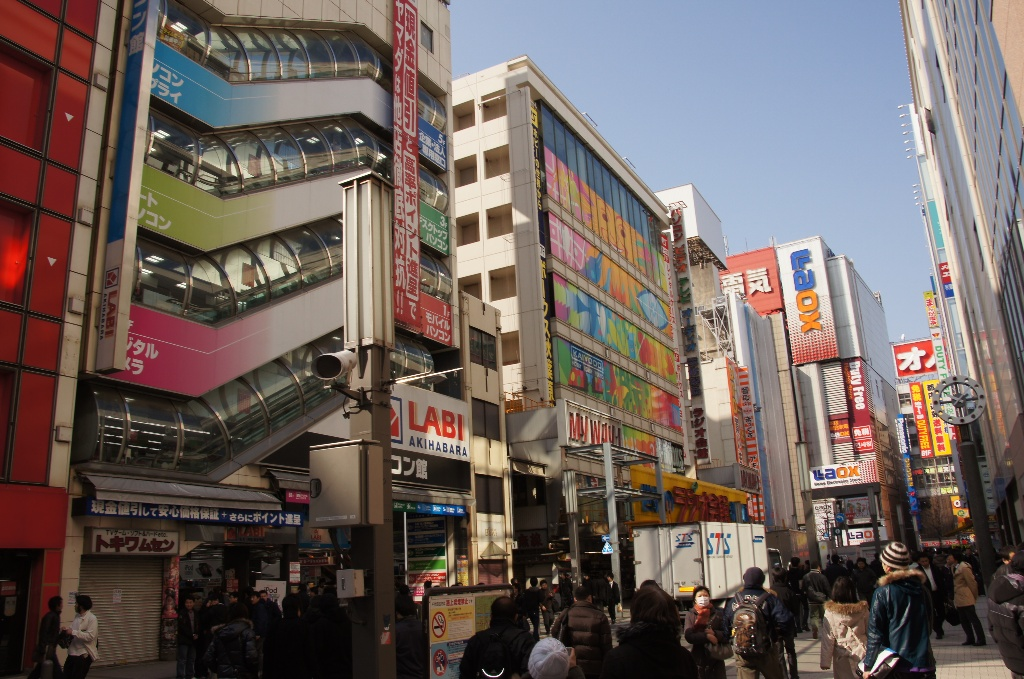
\includegraphics[width=3in]{Akihabara}
\caption{Le quartier d'Akihabara \`a Tokyo.}
\label{fig_akihabara}
\end{figure}

\subsubsection{Impressions}

\begin{figure}[!t]
\centering
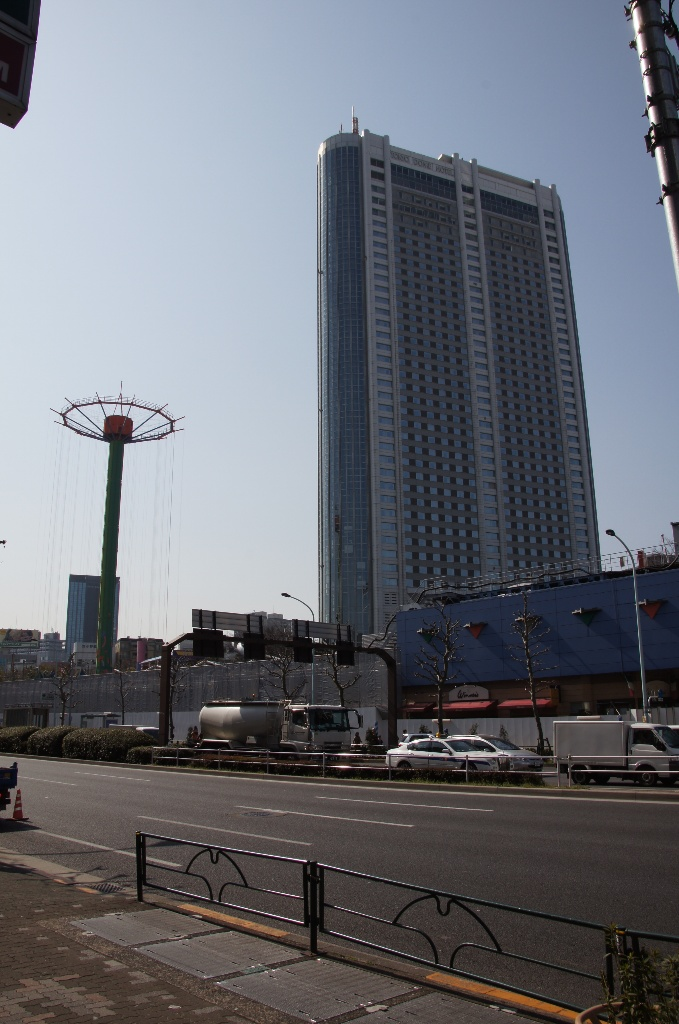
\includegraphics[height=3in]{GrandHotel}
\caption{Le Grand Hotel \`a Tokyo.}
\label{fig_hotel}
\end{figure}

\begin{figure}[!t]
\centering
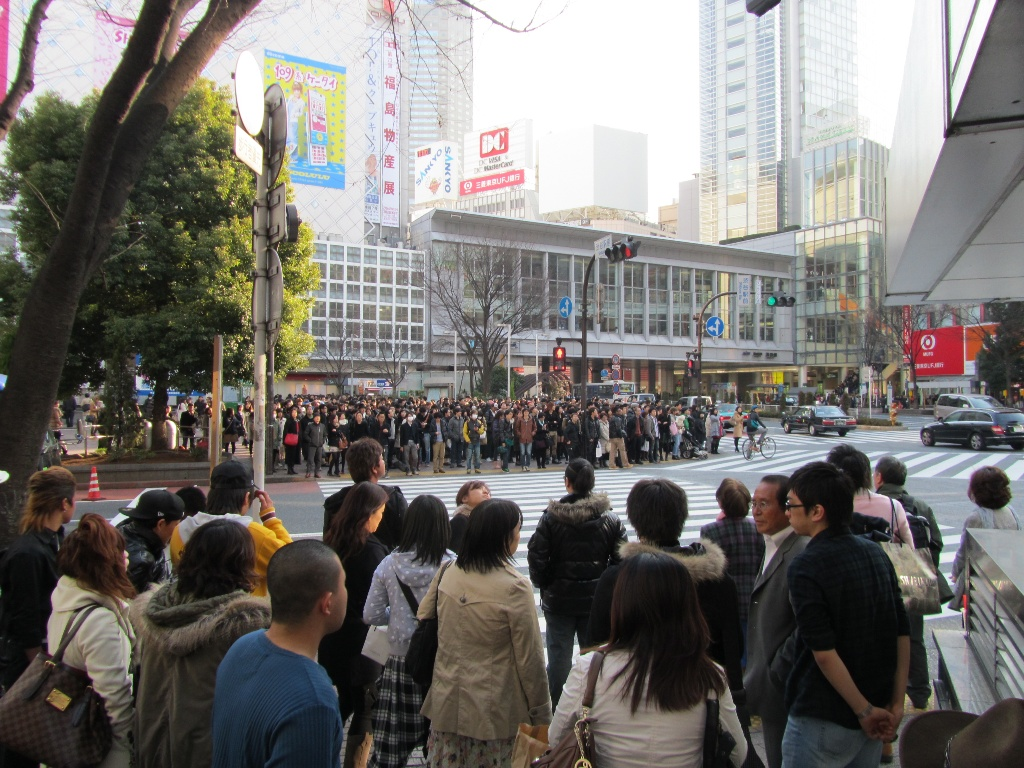
\includegraphics[width=3in]{Shibuya}
\caption{Carrefour de Shibuya avant l'heure de pointe.}
\label{fig_shibuya}
\end{figure}

Si je devais r\'esumer en quelques mots Tokyo je dirais : propre, calme, immense.
Propre, car les gens ne jettent rien dans la rue, les poubelles sont en plus grand nombre qu'en France, mais aussi car les services de propret\'e sont plus pr\'esent et vont jusqu'\`a balayer les parkings pour enlever les feuilles mortes.
Calme, car les Japonais ne parlent pas dans la rue, ou alors tr\`es doucement, le parfait contraste avec les Espagnols que l'on a pu voir par la suite dans la rue en France.
Immense, car tout est d\'emesur\'e, que ce soit la taille de la ville elle-m\^eme ou les batiments, comme le --Grand Hotel-- sur la photo \ref{fig_hotel}. On dirait que les buildings sortent de nulle part. Nous avons \'egalement pu voir le plus grand passage pi\'eton du monde \`a Shibuya pendant l'heure de pointe, il ne faut absolument pas \^etre agoraphobe. La photo \ref{fig_shibuya} a \'et\'e prise avant que nous nous retrouvions coinc\'es dans la mar\'ee humaine.

Tokyo est, d'un autre c\^ot\'e, pourvu de magnifiques parcs qui v\'ehiculent l'image des Japonais, calmes et respectueux, comme celui de la photo \ref{fig_parc}. On y retrouve souvent une v\'eg\'etation surprenante et tr\`es diversifi\'ees et il y r\`egne toujours une atmosph\`ere tr\`es reposante, id\'eale pour se changer les id\'ees.

\begin{figure}[!t]
\centering
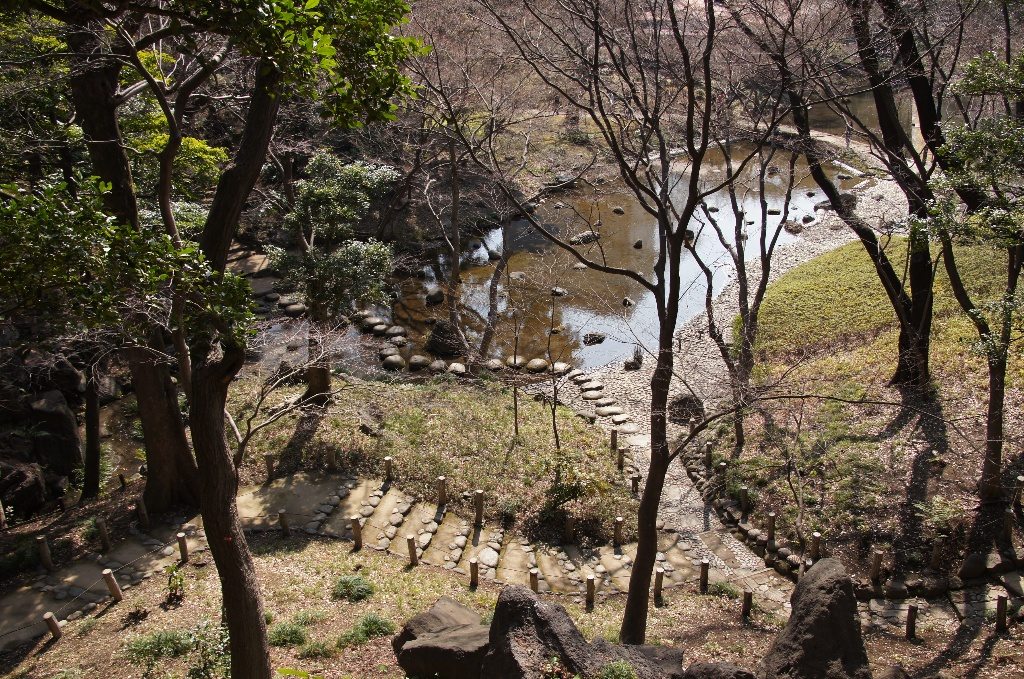
\includegraphics[width=3in]{Parc}
\caption{Le parc Korakuen \`a Tokyo.}
\label{fig_parc}
\end{figure}

\subsubsection{Visites pr\'evues}

\begin{figure}[!t]
\centering
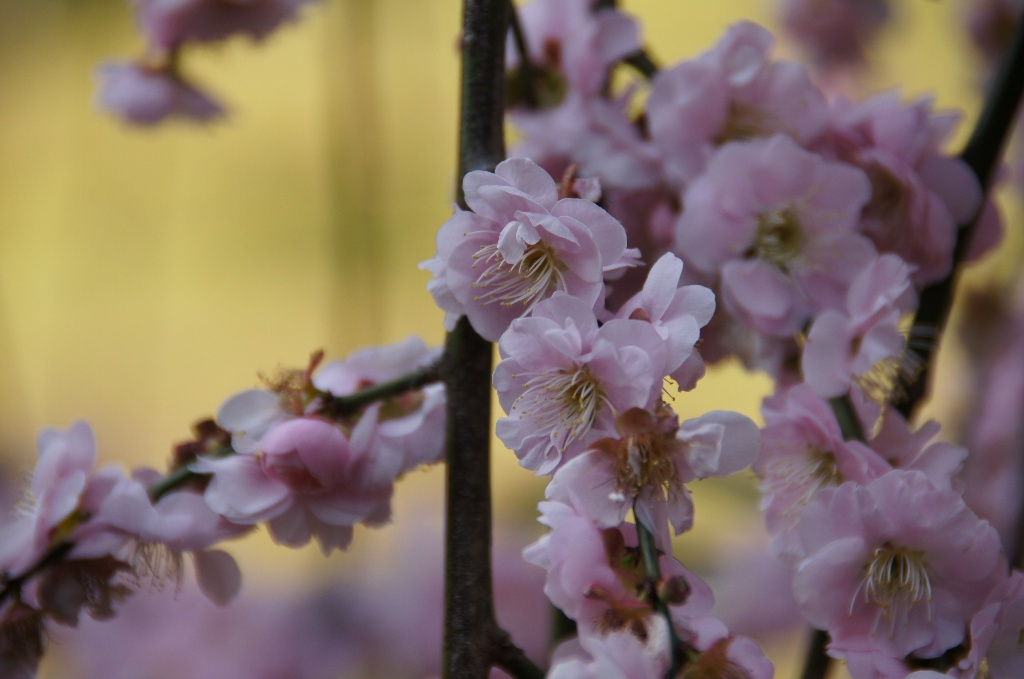
\includegraphics[width=3in]{Sakura}
\caption{D\'ebut de la floraison des cerisiers \`a Tokyo.}
\label{fig_sakura}
\end{figure}

Suite aux incidents que j'aborderai dans la section \ref{sec_incident}, j'ai du \'ecourter mon voyage, me privant ainsi de toutes les visites que j'avais pr\'evues.
En seulement trois week-ends, je n'ai pas eu le temps de visiter grand chose. 
La floraison des cerisiers d\'ebutait juste au moment du d\'epart, je n'ai pas pu assister aux grandes f\^etes nocturnes organis\'ees sous les nuages de p\'etales roses (Photo \ref{fig_sakura}).  

J'avais pos\'e mes vacances pour la semaine suivant le tremblement de terre. Je devais aller visiter tout le sud du Japon \`a l'aide d'un billet de train sp\'ecial : cinq jours de trajets illimit\'es.
Ce voyage pr\'evoyait des escales \`a Nagoya, Kyoto, Nara, et dans d'autres villes moins connues du sud. Je comptais y d\'ecouvrir la culture rurale japonaise, afin de pouvoir comparer avec ce que je voyais tous les jours en ville. Je voulais \'egalement d\'ecouvrir les \textit{Onsen}, les bains d'eau chaude typiquement japonais, et dormir dans un \textit{Ryokan}, un h\^otel traditionnel. Je devrai donc y retourner une fois dipl\^om\'e afin de conna\^\i tre les aspects du Japon que je n'ai pas eu le temps de d\'ecouvrir.




\section{Les Japonais et leur mode de vie} 
\label{sec_mode_de_vie}


\subsection{Coutumes}

Les r\'ev\'erences remplacent les poign\'ees de mains, il faut s'y habituer car les Japonais \'evitent au maximum les contacts. Ils vont donc faire de nombreuses r\'ev\'erences quand ils sont pr\'esent\'es \`a quelqu'un, \`a la limite de l'\'exag\'eration. Dans le m\^eme esprit on retrouve l'omnipr\'esence du $Arigat\bar{o}~ gozaimasu$ (ありがとうございます) signifiant "merci beaucoup". Quand on rentre ou sort d'un magasin, d'un restaurant, dans le m\'etro, le bus, on ne remarque plus que \c{c}a au bout de quelques heures.

D'autre part nous avons rencontr\'e de temps en temps des femmes habill\'ees en costume traditionnel dans les rues de Tokyo ou dans les \'ev\`enements comme sur la photo \ref{fig_music} lors d'un concert de rock \`a Tsukuba. Cette photo exprime bien le m\'elange des coutumes, d'une part transmises par la g\'en\'eration pr\'ec\'edente et celles mises en place par la nouvelle g\'en\'eration.

\begin{figure}[!t]
\centering
\includegraphics[width=3in]{Musique}
\caption{Concert dans les rues de Tsukuba.}
\label{fig_music}
\end{figure}

\subsection{Transports}

\subsubsection{Transport en commun}

Les services de bus sont aussi pr\'esents qu'en France, la grande diff\'erence c'est que l'on paye en descendant et non pas en montant. La fraude n'existe pas ici alors qu'elle est tr\`es pr\'esente en France, le respect joue ici un r\^ole important dans le comportement des Japonais.
Le service des trains est le m\^eme qu'en France \`a l'exception qu'il n'y a jamais de retard, ceci \'etant du \`a la ponctualit\'e exemplaire des Japonais.
Le m\'etro a \'et\'e plus difficile \`a utiliser, car les noms des stations n'\'etaient \'ecrits qu'en Japonais, avec des Kanjis. Nous avons essay\'e de trouver la station \textit{Ochanomizu} (御茶ノ水), mais il a fallu demander de l'aide afin de d\'ecrypter le tableau des destinations.
L'originalit\'e du service de m\'etro est que l'on paye un montant correspondant au traject pr\'evu et que l'on ajuste \`a la sortie aux bornes "\textit{fare adjustment}" si on a \'et\'e plus loin ou plus pr\`es que pr\'evu.
Tous les services de transport en commun sont tr\`es propres et il y r\`egne un climat de s\'ecurit\'e contrairement \`a ce que l'on peut ressentir \`a Paris par exemple. D'autre part la ponctualit\'e des bus/trains/m\'etros est tr\`es appr\'eciable et je comprends mieux pourquoi les Japonais les utilisent \'enorm\'ement.

\subsubsection{Le v\'elo}

Mode de d\'eplacement local par excellence, les Japonais l'utilisent \'enormement, nous avons pu acheter des v\'elos \`a 2000\textyen, soit l'\'equivalent d'une vingtaine d'euros. De nombreuses pistes cyclables et parkings \`a v\'elos sont am\'enag\'es en ville, ce qui rend son utilisation particuli\`erement agr\'eable. Il a cependant fallu un peu de temps pour se faire \`a la conduite \`a gauche qui bouleversait nos habitudes acquises depuis longtemps et qui pouvaient s'av\'erer dangereuses par moments.

Dans un pays o\`u on n'entend presque pas parler d'\'ecologie, j'\'etais content qu'autant de monde utilise des v\'elos, ce qui rendait l'air tr\`es respirable en ville, contrairement aux grandes villes fran\c{c}aises.


\subsection{Commerces}

\subsubsection{Magasins}

A l'oppos\'e de la France, le Japon poss\`ede tr\'es peu de grandes surfaces mais une multitude de petites boutiques. On y retrouve les \textit{7Eleven}, qui sont de petites \'epiceries ouvertes 24h/24 et 7j/7 assez pratiques pour les besoins du quotidien.
Cependant quand il s'agit de trouver des appareils d'\'electrom\'enager, cela devient plus compliqu\'e. Il faut se rendre dans les grandes villes, ou alors s'adresser \`a un des magasins sp\'ecialis\'es qui sont comme en France hors de prix.

\subsubsection{Restaurants}

Presque tous les restaurants proposent en vitrine une reproduction tr\`es r\'ealiste en plastique des plats qu'ils servent, ce qui permet de savoir ou deviner ce que l'on va manger m\^eme si nous ne comprenons pas un seul mot du menu. Un exemple de devanture dans une galerie marchande de Tsukuba, sur la photo \ref{fig_plats}. Certains restaurants vont jusqu'\`a mettre le plat r\'eel du jour sous film plastique. On retrouve des cantines et certains \textit{fast-food} qui utilisent la m\^eme m\'ethode.


\begin{figure}[!t]
\centering
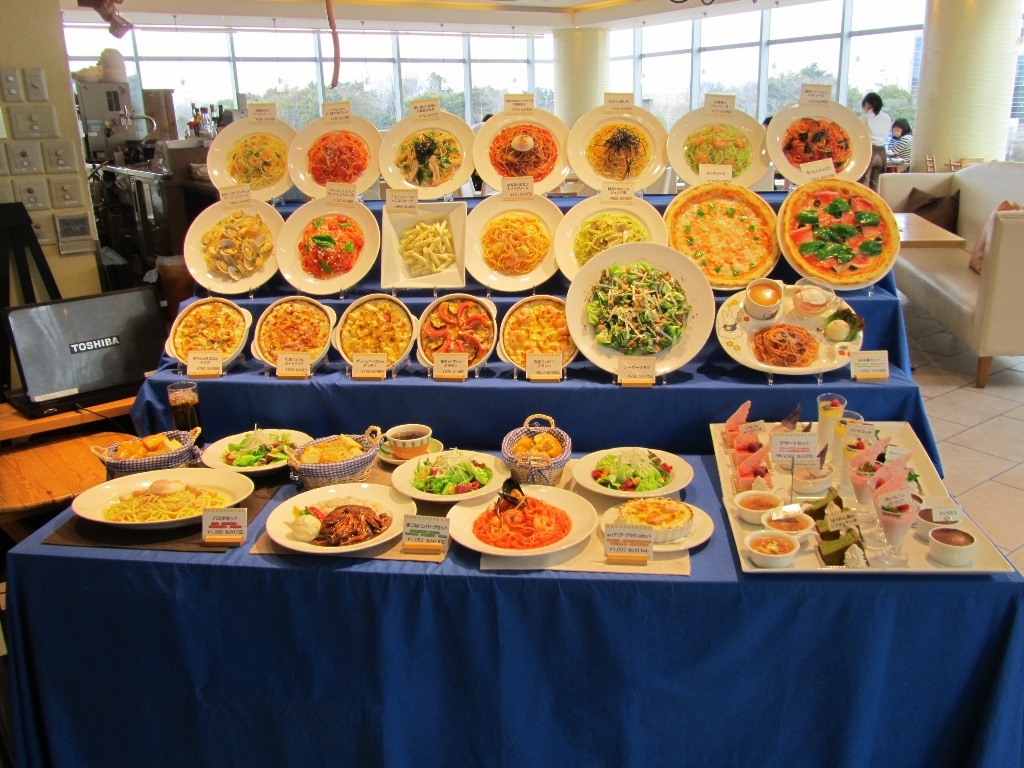
\includegraphics[width=3in]{Plats}
\caption{Vitrine d'un restaurant \`a Tsukuba.}
\label{fig_plats}
\end{figure}

\subsection{Co\^ut de la vie}

On parle souvent du co\^ut \'elev\'e de la vie au Japon, et ce n'est pas qu'une l\'egende. Pour un Europ\'een toute la nourriture est ch\`ere, que ce soit les pommes de terre \`a 70\textyen~l'unit\'e (0,70\texteuro) ou la tomate \`a 140\textyen, la viande \'egalement est ch\`ere, il n'y a que le soja qui soit \`a un prix plus que raisonnable. Au niveau de l'\'electronique on retrouve sensiblement les m\^emes prix qu'en France dans les grandes surfaces de Tokyo. Mais il faut bien se rendre compte que si tout est plus cher, c'est qu'ils sont \'egalement mieux pay\'es, donc pour eux les prix sont tout \`a fait normaux, mais pour les \'etrangers il est souvent compliqu\'e de joindre les deux bouts.

Le loyer est exorbitant, pas moyen de trouver une chambre de 9m carr\'es \`a moins de 500\texteuro/mois en ville, heureusement certaines entreprises poss\`essent leurs propres r\'esidences pour les invit\'es \'etrangers ce qui r\'eduit consid\'erablement les frais.

Les Japonais utilisent assez peu de ch\`eques ou de carte bancaire et pr\'ef\`erent tout payer en liquide, on se retrouve rapidement \`a avoir des dizaine de milliers de yen sur soi pour payer le loyer, le train, les courses et autre. Les distributeurs de l'a\'eroport de Narita ne proposent pas de billet en dessous de 10.000\textyen, l'\'equivalent d'une centaine d'euros.


\section{Les Japonais et leurs contradictions}
\label{sec_contradictions}

\subsection{La t\'el\'evision}

La t\'el\'evision Japonaise est assez particuli\`ere dans le sens o\`u elle contraste totalement avec le reste de la culture.

\subsubsection{Le journal t\'el\'evis\'e}

Le Japon est connu pour \^etre le pays le plus en avance sur la technologie. Cependant en regardant le journal nous pouvons nous rendre compte que les medias ne l'utilisent pas. Alors qu'en France les pr\'esentateurs poss\`edent des \'ecrans int\'eractifs, les Japonais eux, utilisent des posters grands formats sur lesquels ils pr\'esentent les informations \`a l'aide d'une baguette.
Les batailles maritimes (entre la Chine et le Japon) sont expliqu\'ees \`a l'aide de petits bateaux pos\'es sur une carte de la mer de Chine.

L'explication la plus probable \`a cette non-utilisation de la technologie r\'eside dans le fait que les Japonais ont d'avantage confiance aux informations donn\'ees sur format papier. Les posters g\'eant sont donc un moyen d'utiliser cette confiance \`a travers d'autres supports m\'ediatiques.  

\subsubsection{Les jeux t\'el\'evis\'es}

Un autre aspect frappant de la t\'el\'evision Japonais sont les innombrables jeux souvent (tr\`es) pu\'erils. Ceci contraste \'enorm\'ement avec l'image que donnent les Japonais dans la rue, une image d'hommes et de femmes s\'erieux(ses) et irr\'eprochables. 
Serait-ce un moyen de se lib\'erer des pressions accumul\'ees pendant la journ\'ee ? Je pense que c'est \'egalement fait pour retrouver le sourire, une fois chez soi, sorti du monde des convenances. 

\subsection{La nourriture}

Le Japon est r\'eput\'e pour d\'etenir le record de centenaires au monde, ce qui est souvent expliqu\'e par l'\'equilibre des plats Japonais. Cependant la tradition se perd peu \`a peu en raison des \textit{fast-food} et des plats lyophilis\'es dont les Japonais sont grands consommateurs.

Il y a seulement quelques centaines d'ann\'ees, tout le Japon \'etait v\'eg\'etarien pour des raisons de croyances. Cependant \`a cause des importations, cette culture a quasiment disparue, les Japonais mangent d\'esormais \'enorm\'ement de viandes et de poissons. Ceci a un impact visible sur la population qui souffre de probl\`emes de digestion entre autres car leurs corps ne sont pas habitu\'es \`a assimiler ces "nouvelles" substances.

La nourriture a \'et\'e mon gros probl\`eme tout au long du s\'ejour. V\'eg\'etarien depuis ma naissance, je n'ai pas souhait\'e changer pour me mettre \`a l'alimentation Japonaise. Un bon nombre de forums affirmaient qu'il \'etait parfaitement possible de ne pas manger de viande et de poisson au Japon, la r\'ealit\'e \'etait toute autre. Il fallait \`a chaque fois faire plusieurs restaurants avant de trouver un menu avec un plat v\'eg\'etarien, les simples p\^ates \'etant pr\'epar\'ees dans un bouillon de poisson.
Dans les magasins les l\'egumes sont rares et chers, et les c\'er\'erales \'egalement. Nous avons donc essay\'e des l\'egumes de fournisseurs locaux, ダイコン (da\"\i kon),  レンコン  (renkon), 牛蒡 (gobo) qui se sont av\'er\'es d\'elicieux bien que pas forcement tr\`es faciles \`a cuisiner.

%Contrairement aux plats tout pret du commerce


\subsection{Architecture}

\begin{figure}[!t]
\centering
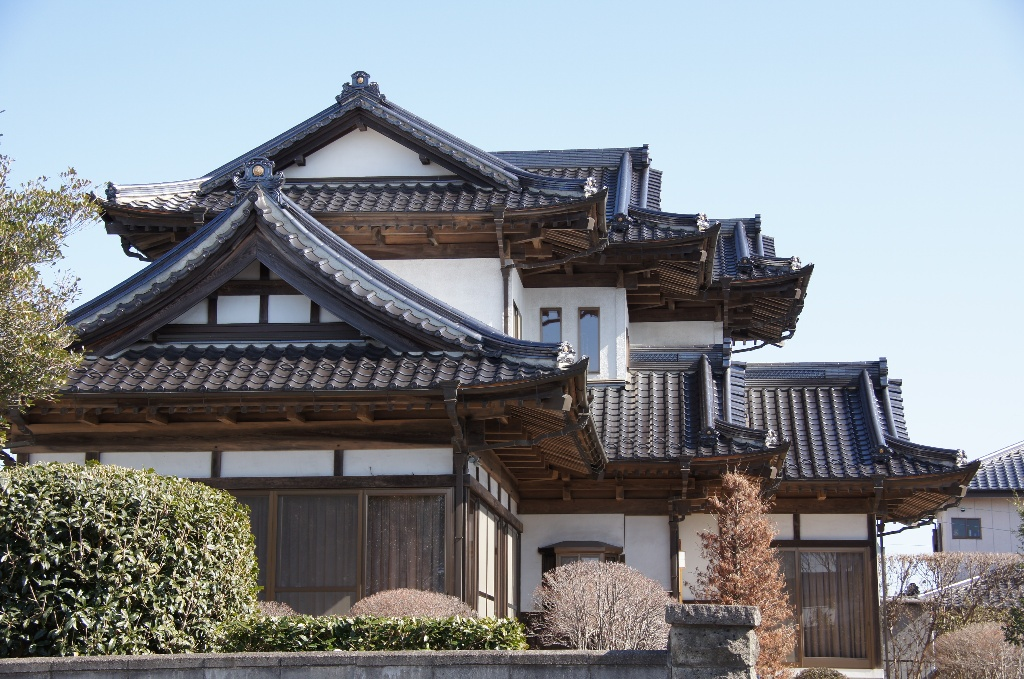
\includegraphics[width=3in]{Maison}
\caption{Une maison traditionnelle \`a Tsuchiura.}
\label{fig_maison}
\end{figure} 

De nombreux tremblements de terre frappent r\'eguli\`erement le Japon et fragilisent peu \`a peu les b\^atiments. Il faut donc r\`eguli\`erement les d\'etruire pour en reconstruire de plus solides et respectant les nouvelles normes sismiques.
\`A cause de ces d\'emolitions permanentes, il y a de moins en moins de maisons traditionnelles comme sur la photo \ref{fig_maison}. Tsukuba est, par exemple, une ville qui m\'elange des HLM, des maisons cubiques en b\'eton, et de magnifique maisons avec des structure en bois. J'ai trouv\'e dommage que l'architecture japonaise disparaisse comme \c{c}a au profit de maisons solides.


On retrouve cependant de nombreux temples cach\'es au milieu des villes comme sur la photo \ref{fig_temple} \`a 500 m\`etres des grands centres commerciaux. Ils sont utilis\'es aussi bien en temps que lieu de culte que de lieu de d\'etente au m\^eme titre que les parcs. On y retrouve donc la totale opposition entre le nouveau Tokyo et l'ancien (Edo). 

\begin{figure}[!t]
\centering
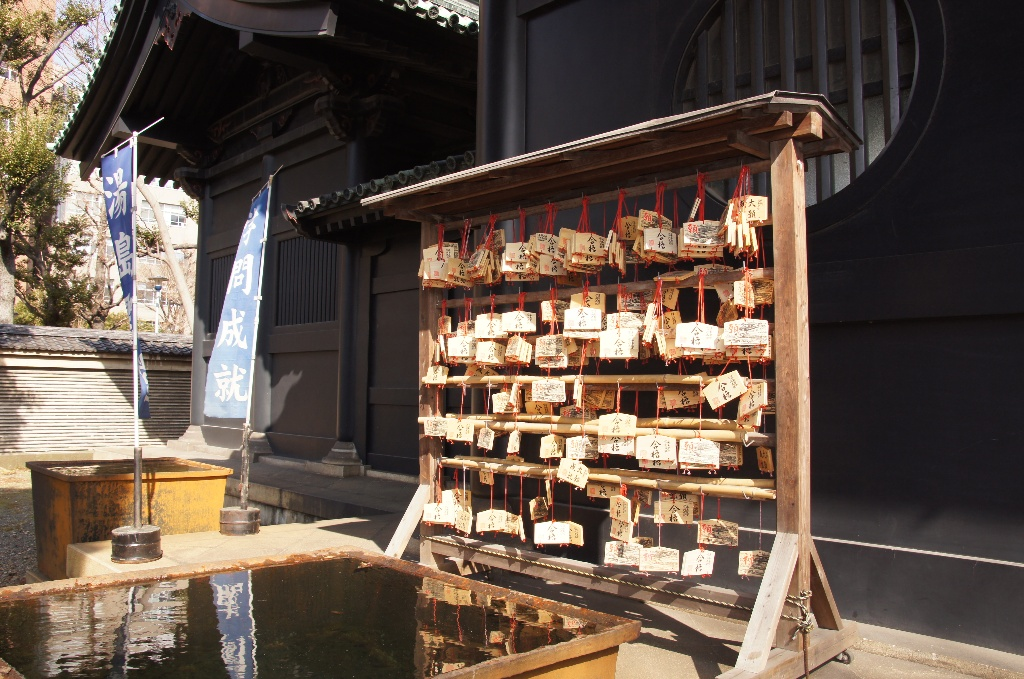
\includegraphics[width=3in]{Temple}
\caption{Un temple dans le quatier d'Ochanomizu.}
\label{fig_temple}
\end{figure}


\section{Incidents : s\'eisme et centrale nucl\'eaire}
\label{sec_incident}
\subsection{Description de l'\'ev\`enement}

Le 11 mars 2011, \`a 13h45 heure locale, un s\'eisme de forte magnitude a frapp\'e le Japon. Il s'est fait ressentir \`a des centaines de kilom\`etres \`a la ronde, comme \`a Tsukuba, \`a 300km de l'\'epicentre. Je travaillais dans le plus grand building du complexe, 8 \'etages ce qui a provoqu\'e de grandes oscillations du batiment. Au troisi\`eme, les armoires bougeaient de plus de 15cm sur place en faisant un bruit inqui\'etant. Les consignes ont vite \'et\'e donn\'ees pour se r\'efugier sous les bureaux en attendant l'accalmie, plus personne n'osait parler.
En sortant quelques minutes apr\`es nous avons pu voir que les armoires avaient \'et\'e renvers\'ees et que les peintures des murs et des plinthes avaient saut\'ees, seulement des d\'egats mineurs en apparence. C'est seulement 3 semaines plus tard que l'on a su que les cloisons du 8{\`eme} s'\'etaient effondr\'ees et qu'il y avait des fissures dans le b\'eton sous les moquettes, de quoi nous couper l'envie d'y retourner.

Pendant plus de 24h il n'y a pas eu d'\'electricit\'e \`a Tsukuba, donc il \'etait impossible de conna\^\i tre l'existence du tsunami ainsi que l'\'etendu relle des d\'egats.

Une fois l'\'electricit\'e revenue nous avons pu regarder les informations \`a la t\'el\'evision japonaise, qui nous parlait d'une centrale nucl\'eaire et montrait des images d'explosions. Mon niveau en japonais ne nous permettait pas de comprendre ce qu'il se passait dans la centrale de Fukushima, \`a 200km de chez nous. Quand nous avons enfin eu internet nous avons eu acc\`es aux informations fran\c caises, qui nous ont fait peur et qui, au bout de quelques heures, nous ont convaincu de fuir le Japon pour quelques jours.
Une fois en France, nous avons appris que tout le personnel fran\c cais du JRL avait fait comme nous.

\begin{figure}[!t]
\centering
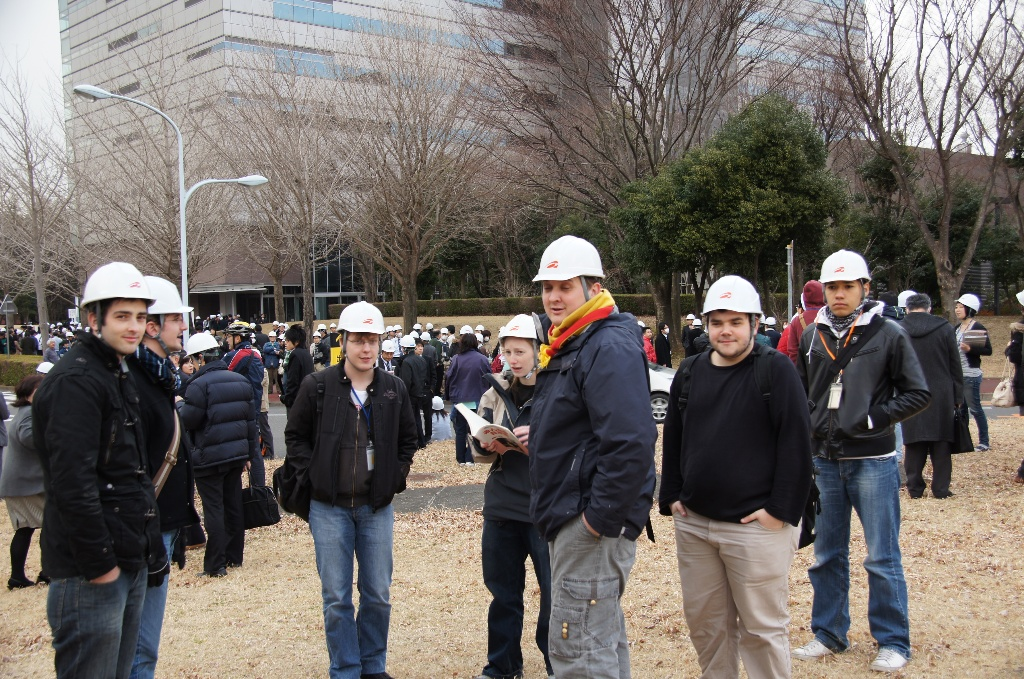
\includegraphics[width=3in]{Earthquake}
\caption{Rassemblement des Fran\c cais apr\`es le tremblement de terre.}
\label{fig_earthquake}
\end{figure}

\subsection{Comportement des Japonais}

Les Japonais \'etaient tr\`es calmes pendant et apr\`es le tremblement de Terre, sans doute par habitude. Les Fran\c cais, eux, \'etait sur le qui-vive en redoutant toujours de fortes r\'epliques, il \'etait donc tr\`es difficile de dormir normalement mais je pense que l'on s'y fait assez rapidement.

Ce qui nous a le plus marqu\'e, c'est la r\'eaction des Japonais face \`a la catastrophe nucl\'eaire. Je devrais plut\^ot dire le manque de r\'eaction car nous avions l'impression qu'ils avaient une confiance aveugle dans les propos rassurants des autorit\'es, qui "maitrisaient" la situation. Seule une amie Japonaise nous a averti des risques de pluies radioactives, mais jamais d'informations officielles...

\subsection{Gouvernements Fran\c cais et Japonais}

Un des Fran\c cais a appel\'e l'ambassade afin de conna\^\i tre les consignes d'urgence. La seule r\'eponse que l'on a pu avoir c'\'etait "\textit{Achetez de l'eau et confinez vous chez vous.}". Cependant les magasins avaient d\'ej\`a \'et\'e d\'evalis\'es, et donc impossible de faire des provisions convenables.
Nous avons ensuite attendu les consignes sur internet comme conseill\'e, mais le site de l'ambassade \'etait inaccessible une fois sur deux. Nous avons appris qu'un avion avait \'et\'e mis \`a disposition pour le rapatriement des femmes enceintes et des enfants en bas \^age uniquement. Il n'y a pas eu d'autre avion gratuit pour le retour en France.
L'impression g\'en\'erale \'etait que l'ambassade nous laissait tomber et qu'il fallait se d\'ebrouiller par nous m\^eme. Nous avons donc tous ressenti que le gouvernement Fran\c cais ne servait \`a rien en cas de catastrophe, ce qui est relativement d\'ecevant quand on est tr\`es stress\'e comme nous l'\'etions tous dans cette situation inhabituelle.

D'autre part les quelques informations donn\'ees au compte-gouttes par le gouvernement Japonais ou l'ambassade de France, \'etaient en contradiction avec tout ce que disaient les m\'edia et les experts \'etrangers. Entre les explosions "\textit{contr\^ol\'ees}", et les r\'eacteurs qui n'ont subi aucun dommage, les mensonges \'etaient si importants que c'est ce qui nous a fait le plus peur.

La pr\'efecture d'Ibaraki est aujourd'hui la deuxi\`eme r\'egion la plus radioactive au Japon, nous sommes donc rassur\'es d'\^etre en France aujourd'hui. Et nous ne pouvons que plaindre tous les Japonais qui n'ont pas pu quitter la r\'egion ou le pays.


\subsection{Cons\'equences}

\`A la suite de cette catastrophe des manifestations ont commenc\'e \`a apparaitre contre le nucl\'eaire. La t\'el\'evision Fran\c{c}aise d\'enombrait seulement une petite dizaine de manifestants pour les premi\`eres car les Japonais ne manifeste jamais en cas g\'en\'eral. Mais elles ont continu\'e et ont abouti \`a la fermeture d'une des centrales jug\'ees dangereuses. C'est donc un tournant tr\`es important pour l'\'ecologie au Japon. 
N'\'etant pas rentr\'e en contact avec des Japonais depuis mon retour, je n'ai pas pu discuter de la fa\c{c}on dont ils ont r\'eagi face \`a cet \'ev\`enement. Toutes les conclusions que j'ai pu formuler sont donc purement hypoth\'etiques. Il aurait \'et\'e int\'eressant de confronter les points de vue des Fran\c{c}ais qui sont partis et des Japonais qui sont rest\'es. Malheureusement la situation ne s'\'etant pas beaucoup am\'elior\'ee, j'ai pr\'ef\'er\'e rester en France pour terminer mon stage.


\section{Conclusion}

En ce qui concerne les sujets que j'aurais pu aborder tel que l'ambiance au travail, la hi\'erarchie dans les entreprises Japonaises ou autres sujets relatifs au travail, je ne peux pas dire que ce soit vraiment diff\'erent des entreprises fran\c{c}aises, l'AIST ressemblant en tout point \`a un complexe scientifique fran\c{c}ais.

N'\'etant rest\'e que 30 jours au Japon, je n'ai pas eu le temps de d\'ecouvrir ou de rencontrer assez de personnes pour que ce rapport puisse contenir tous les \'el\'ements culturels attendus. D'autre part je pense que 3 mois sont insuffisants pour d\'ecouvrir un pays et sa population tout en travaillant 5 jours sur 7.

%J'ai \'et\'e tr\`es surpris et dans un sens un peu d\'e\c cu par le Japon et les Japonais en g\'en\'eral...
%Leurs fa\c con d'agir "comme des moutons" ...

\begin{figure}[!t]
\centering
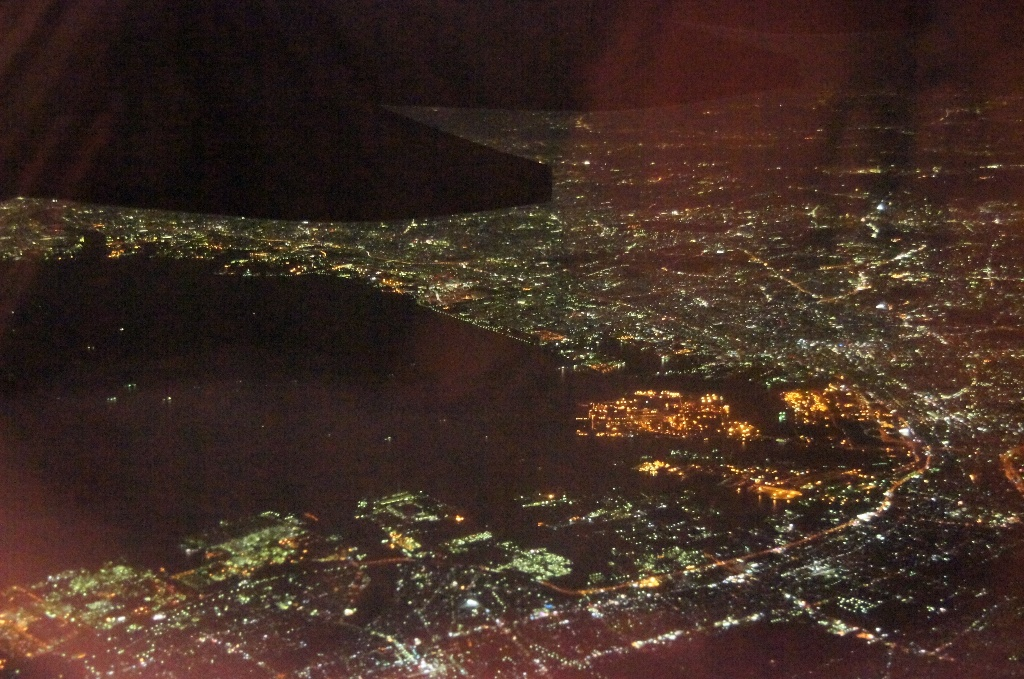
\includegraphics[width=3in]{Depart}
\caption{D\'epart de Tokyo suite aux catastrophes.}
\label{fig_depart}
\end{figure}

La photo \ref{fig_depart} est la derni\`ere image que j'ai du Japon, avec le survol de Tokyo, une ville immense. J'esp\`ere r\'eellement pouvoir y retourner un jour dans de meilleures conditions sismiques.


\section*{Remerciements}


Merci \`a Philippe Martinet de m'avoir mis en contact avec Olivier Stasse et Eiichi Yoshida et permis de travailler dans le domaine de la robotique humano\"\i de. 

Merci \`a Lucie Dejoux\footnote{Qui m'a aid\'e a corriger ce rapport.}, ma compagne, de m'avoir suivi dans l'inconnu \`a l'autre bout du monde sans savoir ce qu'elle allait faire une fois sur place et qui ne s'en est pas trop mal tir\'ee.

Un grand merci \`a Nicolas Perrin, Olivier Stasse, Eiichi Yoshida, Florent Lamiraux, Thomas Moulard\footnote{Ce document a \'et\'e enti\`erement \'edit\'e sous \LaTeX, avec l'aide de Thomas Moulard pour incorporer les caract\`eres japonais.}, Sovannara Hak et toutes les personnes que j'ai pu rencontrer pendant et apr\`es ce voyage.




\end{CJK*}
\end{document}


